\section{Durchführung}
\label{sec:Durchführung}

In dem Versuch soll die Durchbiegung $D(x)$ von drei Stäben in Abhängigkeit vom horizontalen 
Abstand $x$ zum Ort der Einspannung bestimmt werden.
Davon werden zwei Stäbe bei einseitiger Einspannung (einer mit zylindrischem und einer mit 
quadratischem Querschnitt) und ein weiterer bei beidseitiger Einspannung vermessen. 

Die dazu verwendete Apparatur ist in Abbildung \ref{fig:aufbauamk} dargestellt.
\begin{figure}
	\centering
	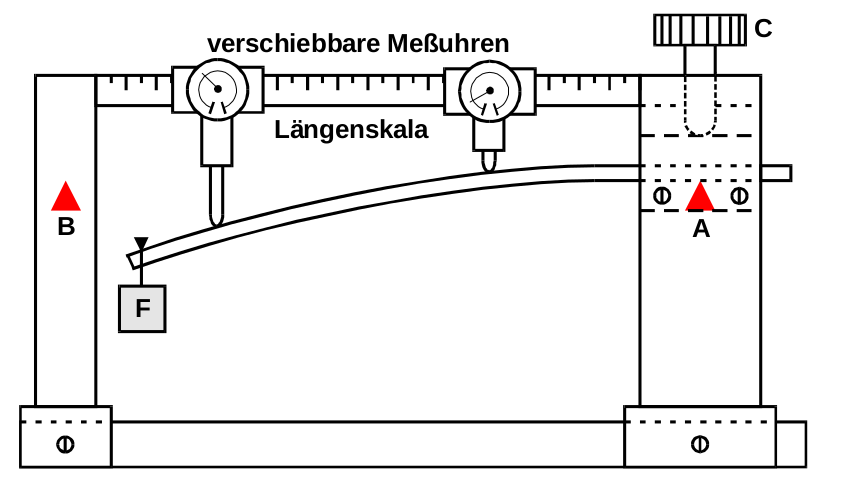
\includegraphics[width=0.7\textwidth]{Bilder/Aufbau_Messung.png}
	\caption{Messapparatur zur Bestimmung der Durchbiegung $D(x)$ in Abhängigkeit von
	Entfernung $x$ zum Einspannungsort. \cite{Anleitung}}
	\label{fig:aufbauamk}
\end{figure}
\subsection{Messung der Durchbiegung eines Stabes bei einseitiger Einspannung}
Für die einseitige Einspannung wird der zu messende Stab in die Spannvorrichtung C geschoben und mit dem Feststellrad befestigt.

Zur Messung der Durchbiegung werden zwei verschiebbare Messuhren verwendet, wobei bei der 
einseitigen Einspannung eine Messuhr genügt. Die zweite Messuhr wird an das andere Ende der
Längenskala verschoben.
Die Messuhren haben einen Messbereich von $\SI{0,01}{\milli\meter}$ bis $\SI{10}{\milli\meter}$.
Weiterhin gibt es zwei Skalen. Auf der kleineren wird der aktuelle Millimeter angezeigt und 
auf der größeren die beiden Nachkommastellen, wobei ein Teilstrich auf der Längenskala 
$\SI{10}{\micro\meter}$ entspricht.
Es wird an jedem Zentimeter auf der Längenskala die Durchbiegung des Stabes an der 
entsprechenden Stelle auf der Messuhr abgelesen.

Für jeden Stab werden zwei Messdurchgänge -- einer ohne Last und einer mit Last -- durchgeführt, 
da nicht von einer exakt symmetrischen Form der Stäbe ausgegangen werden kann und die Eigenmasse 
der Stäbe eine Auslenkung ohne angehängt Last hervorruft.
Damit ergibt sich die effektive Durchbiegung $D(x)$ zu
\begin{equation}
	D(x) = D_{\mathrm{M}}(x) - D_0(x) \mathrm{,}
\end{equation}
mit der Durchbiegung des eingespannten Stabes mit Last $D_{\mathrm{M}}(x)$ und der Durchbiegung
des eingespannten Stabes ohne Last $D_0(x)$.
Hierbei ist zu beachten, dass die Messung ohne Last zuvor durchgeführt wird, um das Phänomen 
der elastischen Nachwirkung \cite{V102} und damit einhergehende Fehler zu vermeiden.

Die Last wird an einer Halterung am nicht eingespannten Ende des Stabes befestigt. Weiterhin 
werden die verwendeten Gewichte über eine Drehschraube befestigt.
Des Weiteren ist die Last so groß zu wählen, dass am Angriffspunkt der Last eine Durchbiegung 
zwischen \SI{3}{\milli\meter} und \SI{7}{\milli\meter} zu messen ist.

\subsection{Messung der Durchbiegung eines Stabes bei zweiseitiger Einspannung}
Zur Messung der zweiseitigen Einspannung wird der zu messende Stab auf die beiden Auflagepunkte 
A und B gelegt.

Weiterhin werden bei dieser Messung beide Messuhren benötigt und die Last wird genau zwischen 
den beiden Messpunkten A und B angebracht. Auch hier ist auf eine Durchbiegung im Bereich 
zwischen \SI{3}{\milli\meter} und \SI{7}{\milli\meter} am Angriffspunkt der Last zu achten.

Der Messvorgang funktioniert analog zur Messung bei einseitig eingespanntem Stab.

\subsection{Ermitteln der Eigenschaften der Stäbe}
Außerdem werden die geometrischen Eigenschaften der Stäbe bestimmt.

Die Länge der Stäbe wird mit einer Schieblehre gemessen.
Weiterhin wird mit einer Mikrometerschraube der Durchmesser der Stäbe bestimmt.
Zuletzt werden mit einer elektronischen Waage die Massen der Stäbe und der angebrachten 
Lasten ermittelt.

